\documentclass{beamer}
%\documentclass[handout]{beamer}

% language settings
%\usepackage{fontspec, polyglossia}
%\setdefaultlanguage{magyar}

% common packages
\usepackage{amsmath, multimedia, hyperref, color, multirow}
%\usepackage{graphicx}

% TikZ
\usepackage{tikz}
%\usetikzlibrary{arrows.meta, decorations.pathmorphing, decorations.pathreplacing, shapes.geometric,mindmap}
%\usetikzlibrary{shapes.geometric,fadings,bayesnet}

% beamer styles
\mode<presentation>{
\usetheme{Madrid}
%\usetheme{Antibes}
\usecolortheme{beaver}
%\usecolortheme{seahorse}
%\usefonttheme{structureitalicserif}
\setbeamercovered{transparent}
}
\setbeamertemplate{blocks}[rounded][shadow=true]
\AtBeginSubsection[]{
  \begin{frame}<beamer>{Contents}
    \tableofcontents[currentsection,currentsubsection]
  \end{frame}
}
%\useoutertheme[]{tree}

% title, etc
\title[Somatic Mutations in the Brain]{Somatic Mutations in the Human Brain from NGS data}
\subtitle{A subtitle may be shorter and more technical}
\author{Attila Guly\'{a}s-Kov\'{a}cs/Jones}
\date{C.~Rosenbluh, A.~Chess}

\begin{document}

\maketitle

\begin{frame}{Genetics of psychiatric disorders}
\begin{itemize}
\item germline variants
\item \textit{de novo} variants
\item<2-> gene-gene and gene-environment interactions  
\item<3-> somatic variants
\begin{itemize}
%\item<3-> \alert{our hypothesis: psychiatric disorders; schizophrenia}
\item cancer, aging
\item V(D)J recombination
\item dysplasias: hemimegencephaly, lissencephaly, pediatric epilepsy 
\item<4-> \alert{neurological and psychiatric disorders?}
\end{itemize}
\end{itemize}
\end{frame}

\begin{frame}
\includegraphics[height=0.8\textheight]{figures/from-others/bsm-science-fig1.jpg}
\end{frame}

\begin{frame}[label=bsm-methods]{Sequencing approaches to detect somatic variants}
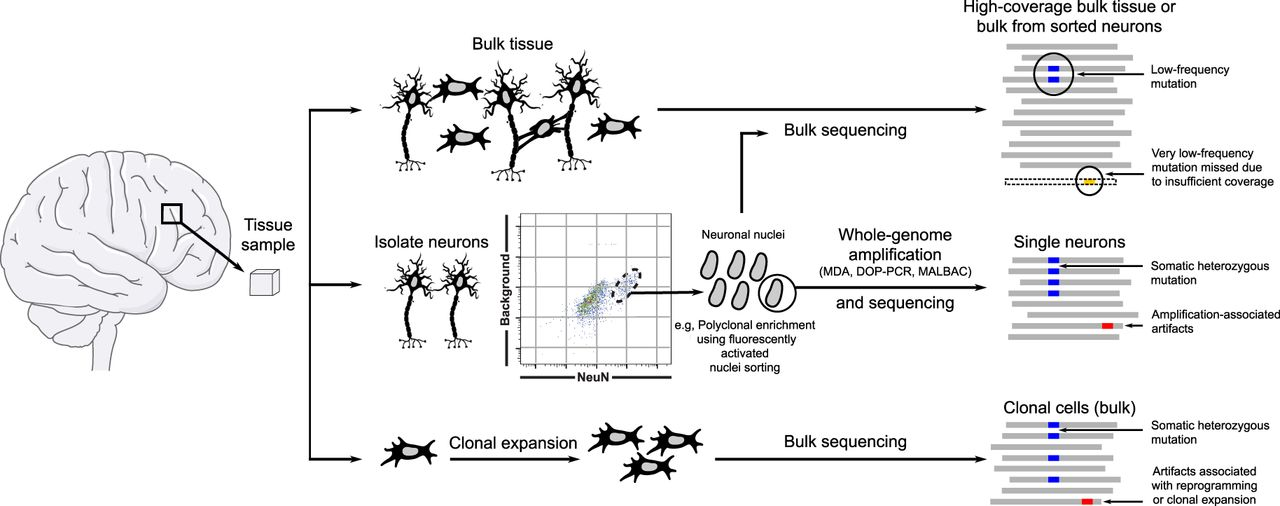
\includegraphics[width=1.0\textwidth]{figures/from-others/bsm-science-fig2.jpg}
\end{frame}

\begin{frame}{Proposed functional validation}
\includegraphics[width=1.0\textwidth]{figures/from-others/bsm-science-fig4.jpg}
\end{frame}

\begin{frame}{Patterns of somatic mosaicism}
\includegraphics[width=1.0\textwidth]{figures/from-others/lodato2015science-fig3ab.png}
\end{frame}

\begin{frame}{Embryonic development}
%gastrulation video
%https://www.youtube.com/watch?v=3AOoikTEfeo
%neurulation video
%https://www.youtube.com/watch?v=lGLexQR9xGs
\includegraphics[height=0.8\textheight]{figures/from-others/HumanEmbryogenesis.png}
\end{frame}

\begin{frame}{Neocortical development}
\includegraphics[height=0.8\textheight]{figures/from-others/doi_10_1016-j_cell_2011_06_030-fig4b-neocortical-development.jpg}
\end{frame}

\begin{frame}{Mutation rate}
\includegraphics[width=0.8\columnwidth]{figures/from-others/lynch-evolution-of-mutation-rate-fig3.jpg}
\end{frame}

\againframe{bsm-methods}

\begin{frame}[label=data-quantity]{Samples and NGS data}
\includegraphics[height=0.85\textheight]{figures/2017-05-24-alignment-stats/combined-depth-plot-1.png}
\end{frame}

\begin{frame}{Ongoing analyses}
\includegraphics[width=1.0\columnwidth]{figures/2018-09-12-sequenced-individuals/summary-cmc-1.pdf}
\end{frame}

\begin{frame}{Discordance between variant callers}

\begin{columns}[t]
\begin{column}{0.5\textwidth}

\includegraphics<1-2>[width=1.0\columnwidth]{figures/2018-10-26-MSSM106-control-indiv/call-set-size-snvs-1.pdf}
\includegraphics<3>[width=1.0\columnwidth]{figures/2018-10-26-MSSM106-control-indiv/call-set-size-snvs-2.pdf}
\end{column}

\begin{column}{0.6\textwidth}

\includegraphics<2>[width=1.0\columnwidth]{figures/2018-10-26-MSSM106-control-indiv/venn-snvs-1.pdf}
\includegraphics<3>[width=1.0\columnwidth]{figures/2018-10-26-MSSM106-control-indiv/venn-snvs-PASS-1.pdf}
\end{column}
\end{columns}
\end{frame}

\begin{frame}{Heuristic filtering and combination of call sets}
\tiny
\setlength{\tabcolsep}{3pt}
\begin{tabular}{l|llllllll|}
\footnotesize &
\multicolumn{8}{c}{\footnotesize \texttt{TNseq.Mutect2.vcf}} \\
\hline
 & \#CHROM & POS & ID & REF & ALT & QUAL & FILTER & INFO \\
\textcolor{cyan}{\(c\)} &
\textcolor{cyan}{1} &
\textcolor{cyan}{50003788} &
\textcolor{cyan}{0} &
\textcolor{cyan}{A} &
\textcolor{cyan}{G} &
\textcolor{cyan}{0} &
\textcolor{cyan}{t\_lod\_fstar} &
\textcolor{cyan}{...;NLOD=30.4;TLOD=4.62} \\
\textcolor{cyan!50!brown}{\(d\)} &
\textcolor{cyan!50!brown}{1} &
\textcolor{cyan!50!brown}{50005034} &
\textcolor{cyan!50!brown}{0} &
\textcolor{cyan!50!brown}{G} &
\textcolor{cyan!50!brown}{T} &
\textcolor{cyan!50!brown}{0} &
\textcolor{cyan!50!brown}{t\_lod\_fstar} &
\textcolor{cyan!50!brown}{...;NLOD=33.27;TLOD=4.51} \\
\textcolor{cyan!50!brown}{\(e\)} &
\textcolor{cyan!50!brown}{1} &
\textcolor{cyan!50!brown}{50007349} &
\textcolor{cyan!50!brown}{0} &
\textcolor{cyan!50!brown}{C} &
\textcolor{cyan!50!brown}{T} &
\textcolor{cyan!50!brown}{0} &
\textcolor{cyan!50!brown}{PASS} &
\textcolor{cyan!50!brown}{...;NLOD=23.43;TLOD=10.97} \\
\textcolor{cyan!50!brown}{\(f\)} &
\textcolor{cyan}{1} &
\textcolor{cyan}{50008565} &
\textcolor{cyan}{0} &
\textcolor{cyan}{C} &
\textcolor{cyan}{A} &
\textcolor{cyan}{0} &
\textcolor{cyan}{PASS} &
\textcolor{cyan}{...;NLOD=7.69;TLOD=8.26} \\
\hline
% \vdots & \vdots & \vdots & \vdots & \vdots & \vdots & \vdots & \vdots & \vdots & \vdots & \vdots \\
\end{tabular}
\tiny
\\[1em]
\begin{tabular}{l|llllllll|}
\footnotesize &
\multicolumn{8}{c}{\footnotesize \texttt{strelka2Somatic.vcf}} \\
\hline
 & \#CHROM & POS & ID & REF & ALT & QUAL & FILTER & INFO \\
\textcolor{brown}{\(a\)} &
\textcolor{brown}{1} &
\textcolor{brown}{50003323} &
\textcolor{brown}{0} &
\textcolor{brown}{A} &
\textcolor{brown}{G} &
\textcolor{brown}{0} &
\textcolor{brown}{LowEVS} &
\textcolor{brown}{...;DP=274;MQ=59.86;...;SomaticEVS=0} \\
\textcolor{brown}{\(b\)} &
\textcolor{brown}{1} &
\textcolor{brown}{50003455} &
\textcolor{brown}{0} &
\textcolor{brown}{C} &
\textcolor{brown}{T} &
\textcolor{brown}{0} &
\textcolor{brown}{LowEVS} &
\textcolor{brown}{...;DP=226;MQ=59.9;...;SomaticEVS=0.65} \\
\textcolor{brown}{\(d\)} &
\textcolor{cyan!50!brown}{1} &
\textcolor{cyan!50!brown}{50005034} &
\textcolor{cyan!50!brown}{0} &
\textcolor{cyan!50!brown}{G} &
\textcolor{cyan!50!brown}{T} &
\textcolor{cyan!50!brown}{0} &
\textcolor{cyan!50!brown}{PASS} &
\textcolor{cyan!50!brown}{...;DP=278;MQ=59.95;...;SomaticEVS=9.04} \\
\textcolor{brown}{\(e\)} &
\textcolor{cyan!50!brown}{1} &
\textcolor{cyan!50!brown}{50007349} &
\textcolor{cyan!50!brown}{0} &
\textcolor{cyan!50!brown}{C} &
\textcolor{cyan!50!brown}{T} &
\textcolor{cyan!50!brown}{0} &
\textcolor{cyan!50!brown}{LowEVS} &
\textcolor{cyan!50!brown}{...;DP=192;MQ=59.88;...;SomaticEVS=4.19} \\
\hline
% \vdots & \vdots & \vdots & \vdots & \vdots & \vdots & \vdots & \vdots & \vdots & \vdots & \vdots \\
\end{tabular}
% ##INFO=<ID=SomaticEVS,Number=1,Type=Float,Description="Somatic Empirical
% Variant Score (EVS) expressing the phred-scaled probability of thecall being
% a false positive observation.">
\normalsize


\includegraphics[height=0.6\textheight]{figures/Tnseq-4-strelka2Somatic-4-venn.png}
\end{frame}

\begin{frame}{Discordance in Common Experiment}
\includegraphics[height=0.7\columnwidth]{figures/from-others/bsmn-cs-callset-concordance.png}

\tiny{Brain Somatic Mosaicism Network, unpublished}
\end{frame}

\begin{frame}{Optimizing calling approach}
\begin{columns}[t]
\begin{column}{0.5\textwidth}
consortium
\begin{enumerate}
\item real data set
\item heuristic filtering and combination of call sets
\item validate some calls with targeted resequencing 
\item refine heuristics
\item ...  
\item publish paper \& software
\end{enumerate}
\end{column}

\begin{column}{0.5\textwidth}
our group
\begin{enumerate}
\item benchmark data set with known variants
\item select annotations in call sets
\item input to machine learning\footnote{VariantMetaCaller}
\item validate all calls
\item re-select annotations 
\item ...
\end{enumerate}
\end{column}
\end{columns}
\end{frame}

\begin{frame}[label=benchmark]{Mixed germline variants for benchmarking}
\begin{center}
\begin{columns}[t]
\begin{column}{0.5\textwidth}

\includegraphics[width=1\textwidth]{figures/from-others/ceph-utah-pedigree-1463.png}
\end{column}

\begin{column}{0.5\textwidth}

\small
{\onslide<1->
\begin{tabular}{cccc}
genome & mix1 & mix2 & mix3\\
\hline
NA12889 & 4 & 2 & 0\\
NA12891 & 8 & 4 & 0\\
NA12890 & 16 & 8 & 0\\
NA12892 & 72 & 86 & 100\\
\hline
total & 100 & 100 & 100\\
\end{tabular}
}
\end{column}
\end{columns}
\end{center}
\end{frame}

\begin{frame}{Controlling precision}
\[\mathrm{precision} = 1 - \mathrm{FDR}\]
\begin{columns}[t]
\begin{column}{0.5\textwidth}
\begin{center}
without control
\end{center}
\includegraphics<1-2>[width=1\columnwidth]{figures/by-me/precision-recall/pr-realistic.pdf}
\end{column}

\begin{column}{0.5\textwidth}
\begin{center}
\only<2>{with control }
\end{center}
\includegraphics<2>[width=1\columnwidth]{figures/by-me/precision-recall/pr.pdf}
\end{column}
\end{columns}
\end{frame}

\begin{frame}[label=precrecall]{Callers in precision-recall space}
\includegraphics[width=1\textwidth]{figures/from-others/chaggai-precision-recall.png}

\tiny{Chaggai Rosenbluh}
\end{frame}

\begin{frame}{Impact of alternative allele frequency}
\includegraphics[width=0.9\textwidth]{figures/from-others/chaggai-recall-aaf.png}

\tiny{Chaggai Rosenbluh}
\end{frame}

\againframe{data-quantity}

\begin{frame}{Summary}
\begin{enumerate}
\item \alert{somatic mutations} in neurological psychiatric disorders\\
\emph{Brain Somatic Mosaicism Network}
\item somatic mutations in \alert{schizoprhenic} and control brains\\
\emph{our group}
\item workflows for somatic variant calling: \alert{discordance}
\item workflow characterization and \alert{optimization}
\begin{itemize}
\item heuristics---\emph{BSMN}
\begin{itemize}
\end{itemize}
\end{itemize}
\item probabilistic approach---\emph{our group}
\begin{itemize}
\item benchmark data \(\Rightarrow\) precision--recall
\item \alert{machine learning}
\item input: base/mapping/calling \alert{quality annotations}
\end{itemize}
\end{enumerate}
\end{frame}

\begin{frame}{BSMN consortium team}
Brain Somatic Mosaicism Network
\footnotesize
\begin{tabular}{rl}
\hline
P.I. & institution \\
\hline
Akbarian & Icahn School of Medicine at Mount Sinai\\
Chess & Icahn School of Medicine at Mount Sinai\\
Gage & Salk Institute for Biological Studies\\
Gleeson & University of California, San Diego\\
Moran & University of Michigan\\
Park & Harvard University\\
Pevsner & Kennedy Krieger Institute\\
Sestan & Yale University\\
Vaccarino & Yale University\\
Walsh & Boston Children's Hospital\\
Weinberger & Lieber Institute for Brain Development\\
\end{tabular}
\vfill
\begin{columns}[t]
\begin{column}{0.3\textwidth}
\begin{center}

\includegraphics[width=0.5\columnwidth]{figures/from-others/NIH_logo.png}
\end{center}
\end{column}

\begin{column}{0.3\textwidth}
\begin{center}

\includegraphics[width=0.5\columnwidth]{figures/from-others/nda.pdf}

NIMH Data Archive
\end{center}
\end{column}

\begin{column}{0.3\textwidth}
\begin{center}

\includegraphics[width=0.5\columnwidth]{figures/from-others/synapse.pdf}

Synapse
\end{center}
\end{column}
\end{columns}
\end{frame}
\end{document}


\begin{columns}[t]
\begin{column}{0.5\textwidth}

\end{column}

\begin{column}{0.5\textwidth}

\end{column}
\end{columns}
